\documentclass[10pt]{article}
\usepackage[paperwidth=94mm,paperheight=59mm,margin=1mm]{geometry}
\usepackage{newtxtext,newtxmath,tikz,pgfplots}
\pgfplotsset{compat=1.18}
\definecolor{methodblue}{HTML}{216A85}
\definecolor{controlgray}{HTML}{555555}
\definecolor{accentorange}{HTML}{A64B1D}
\pagestyle{empty}
\begin{document}
\noindent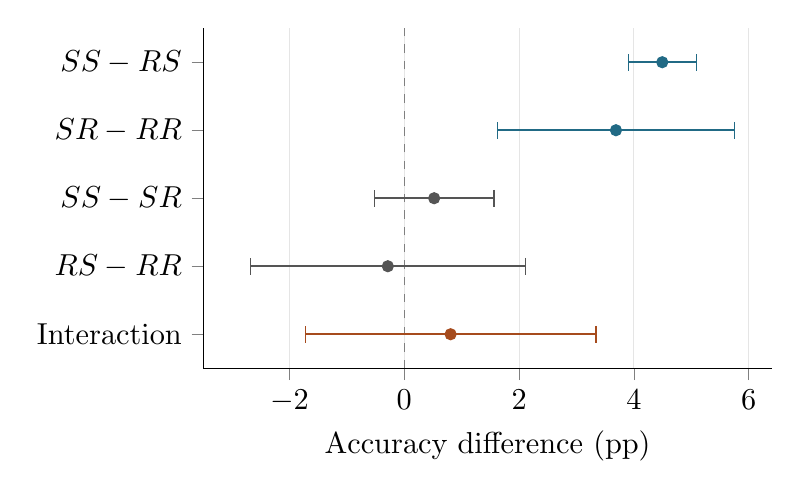
\begin{tikzpicture}
\begin{axis}[width=88mm,height=59mm,xmin=-3.5,xmax=6.4,ymin=-0.5,ymax=4.5,
 xtick={-2,0,2,4,6},ytick={0,1,2,3,4},
 yticklabels={Interaction,$RS-RR$,$SS-SR$,$SR-RR$,$SS-RS$},
 tick label style={font=\fontsize{11}{13}\selectfont},label style={font=\fontsize{11}{13}\selectfont},
 xlabel={Accuracy difference (pp)},axis x line*=bottom,axis y line*=left,
 xmajorgrids=true,grid style={gray!20},tick align=outside]
\draw[dashed,gray] (axis cs:0,-.5)--(axis cs:0,4.5);
\addplot+[only marks,mark=*,mark size=2pt,color=methodblue,mark options={fill=methodblue,draw=methodblue},error bars/.cd,x dir=both,x explicit,error bar style={line width=.8pt},error mark options={rotate=90,mark size=3pt}] coordinates {(4.493333558241531,4) +- (0.5927320398622475,0)};
\addplot+[only marks,mark=*,mark size=2pt,color=methodblue,mark options={fill=methodblue,draw=methodblue},error bars/.cd,x dir=both,x explicit,error bar style={line width=.8pt},error mark options={rotate=90,mark size=3pt}] coordinates {(3.68666611115138,3) +- (2.066069827756956,0)};
\addplot+[only marks,mark=*,mark size=2pt,color=controlgray,mark options={fill=controlgray,draw=controlgray},error bars/.cd,x dir=both,x explicit,error bar style={line width=.8pt},error mark options={rotate=90,mark size=3pt}] coordinates {(0.5200004180272421,2) +- (1.0433379333136656,0)};
\addplot+[only marks,mark=*,mark size=2pt,color=controlgray,mark options={fill=controlgray,draw=controlgray},error bars/.cd,x dir=both,x explicit,error bar style={line width=.8pt},error mark options={rotate=90,mark size=3pt}] coordinates {(-0.28666702906290925,1) +- (2.3978461067738848,0)};
\addplot+[only marks,mark=*,mark size=2pt,color=accentorange,mark options={fill=accentorange,draw=accentorange},error bars/.cd,x dir=both,x explicit,error bar style={line width=.8pt},error mark options={rotate=90,mark size=3pt}] coordinates {(0.8066674470901513,0) +- (2.531545956104275,0)};
\end{axis}\end{tikzpicture}\end{document}
